\chapter{Results and Conclusion}

\section{Evaluation Summary}
The final ResNet-50 baseline was evaluated on a test set containing 1500 samples. Quantitative outcomes are summarized in Table \ref{tab:overall-metrics}.

\begin{table}[h]
\centering
\caption{Overall test performance of DeepSceneLoc Stage 1}
\label{tab:overall-metrics}
\begin{tabular}{lc}
\toprule
Metric & Value \\
\midrule
Overall Accuracy & 0.9233 \\
Macro Precision & 0.9245 \\
Macro Recall & 0.9233 \\
Macro F1-score & 0.9237 \\
Total Samples & 1500 \\
\bottomrule
\end{tabular}
\end{table}

\section{Class Wise Performance}
Table \ref{tab:class-metrics} reports class-level metrics.

\begin{table}[h]
\centering
\caption{Per-class performance metrics}
\label{tab:class-metrics}
\begin{tabular}{lcccc}
\toprule
Class & Accuracy & Precision & Recall & F1-score \\
\midrule
Coastal & 0.9033 & 0.8885 & 0.9033 & 0.8959 \\
Forest & 0.9700 & 0.9798 & 0.9700 & 0.9749 \\
Mountain & 0.8700 & 0.8339 & 0.8700 & 0.8515 \\
Rural & 0.9833 & 0.9833 & 0.9833 & 0.9833 \\
Urban & 0.8900 & 0.9368 & 0.8900 & 0.9128 \\
\bottomrule
\end{tabular}
\end{table}

\section{Confusion Analysis}
The confusion matrix indicates that the model performs strongly on Rural and Forest scenes, while the Mountain class shows the highest overlap with Coastal and Urban categories. This is expected because these classes can share visual patterns such as rocky textures, skyline segments, or sparse built structures.

\begin{table}[htbp]
\centering
\caption{Top off-diagonal confusion pairs from test predictions}
\label{tab:top-confusions}
\begin{tabular}{l l c}
\toprule
True Class & Predicted Class & Count \\
\midrule
Coastal & Mountain & 24 \\
Mountain & Coastal & 22 \\
Urban & Mountain & 21 \\
Mountain & Urban & 10 \\
Urban & Coastal & 8 \\
\bottomrule
\end{tabular}
\end{table}

\begin{figure}[htbp]
\centering
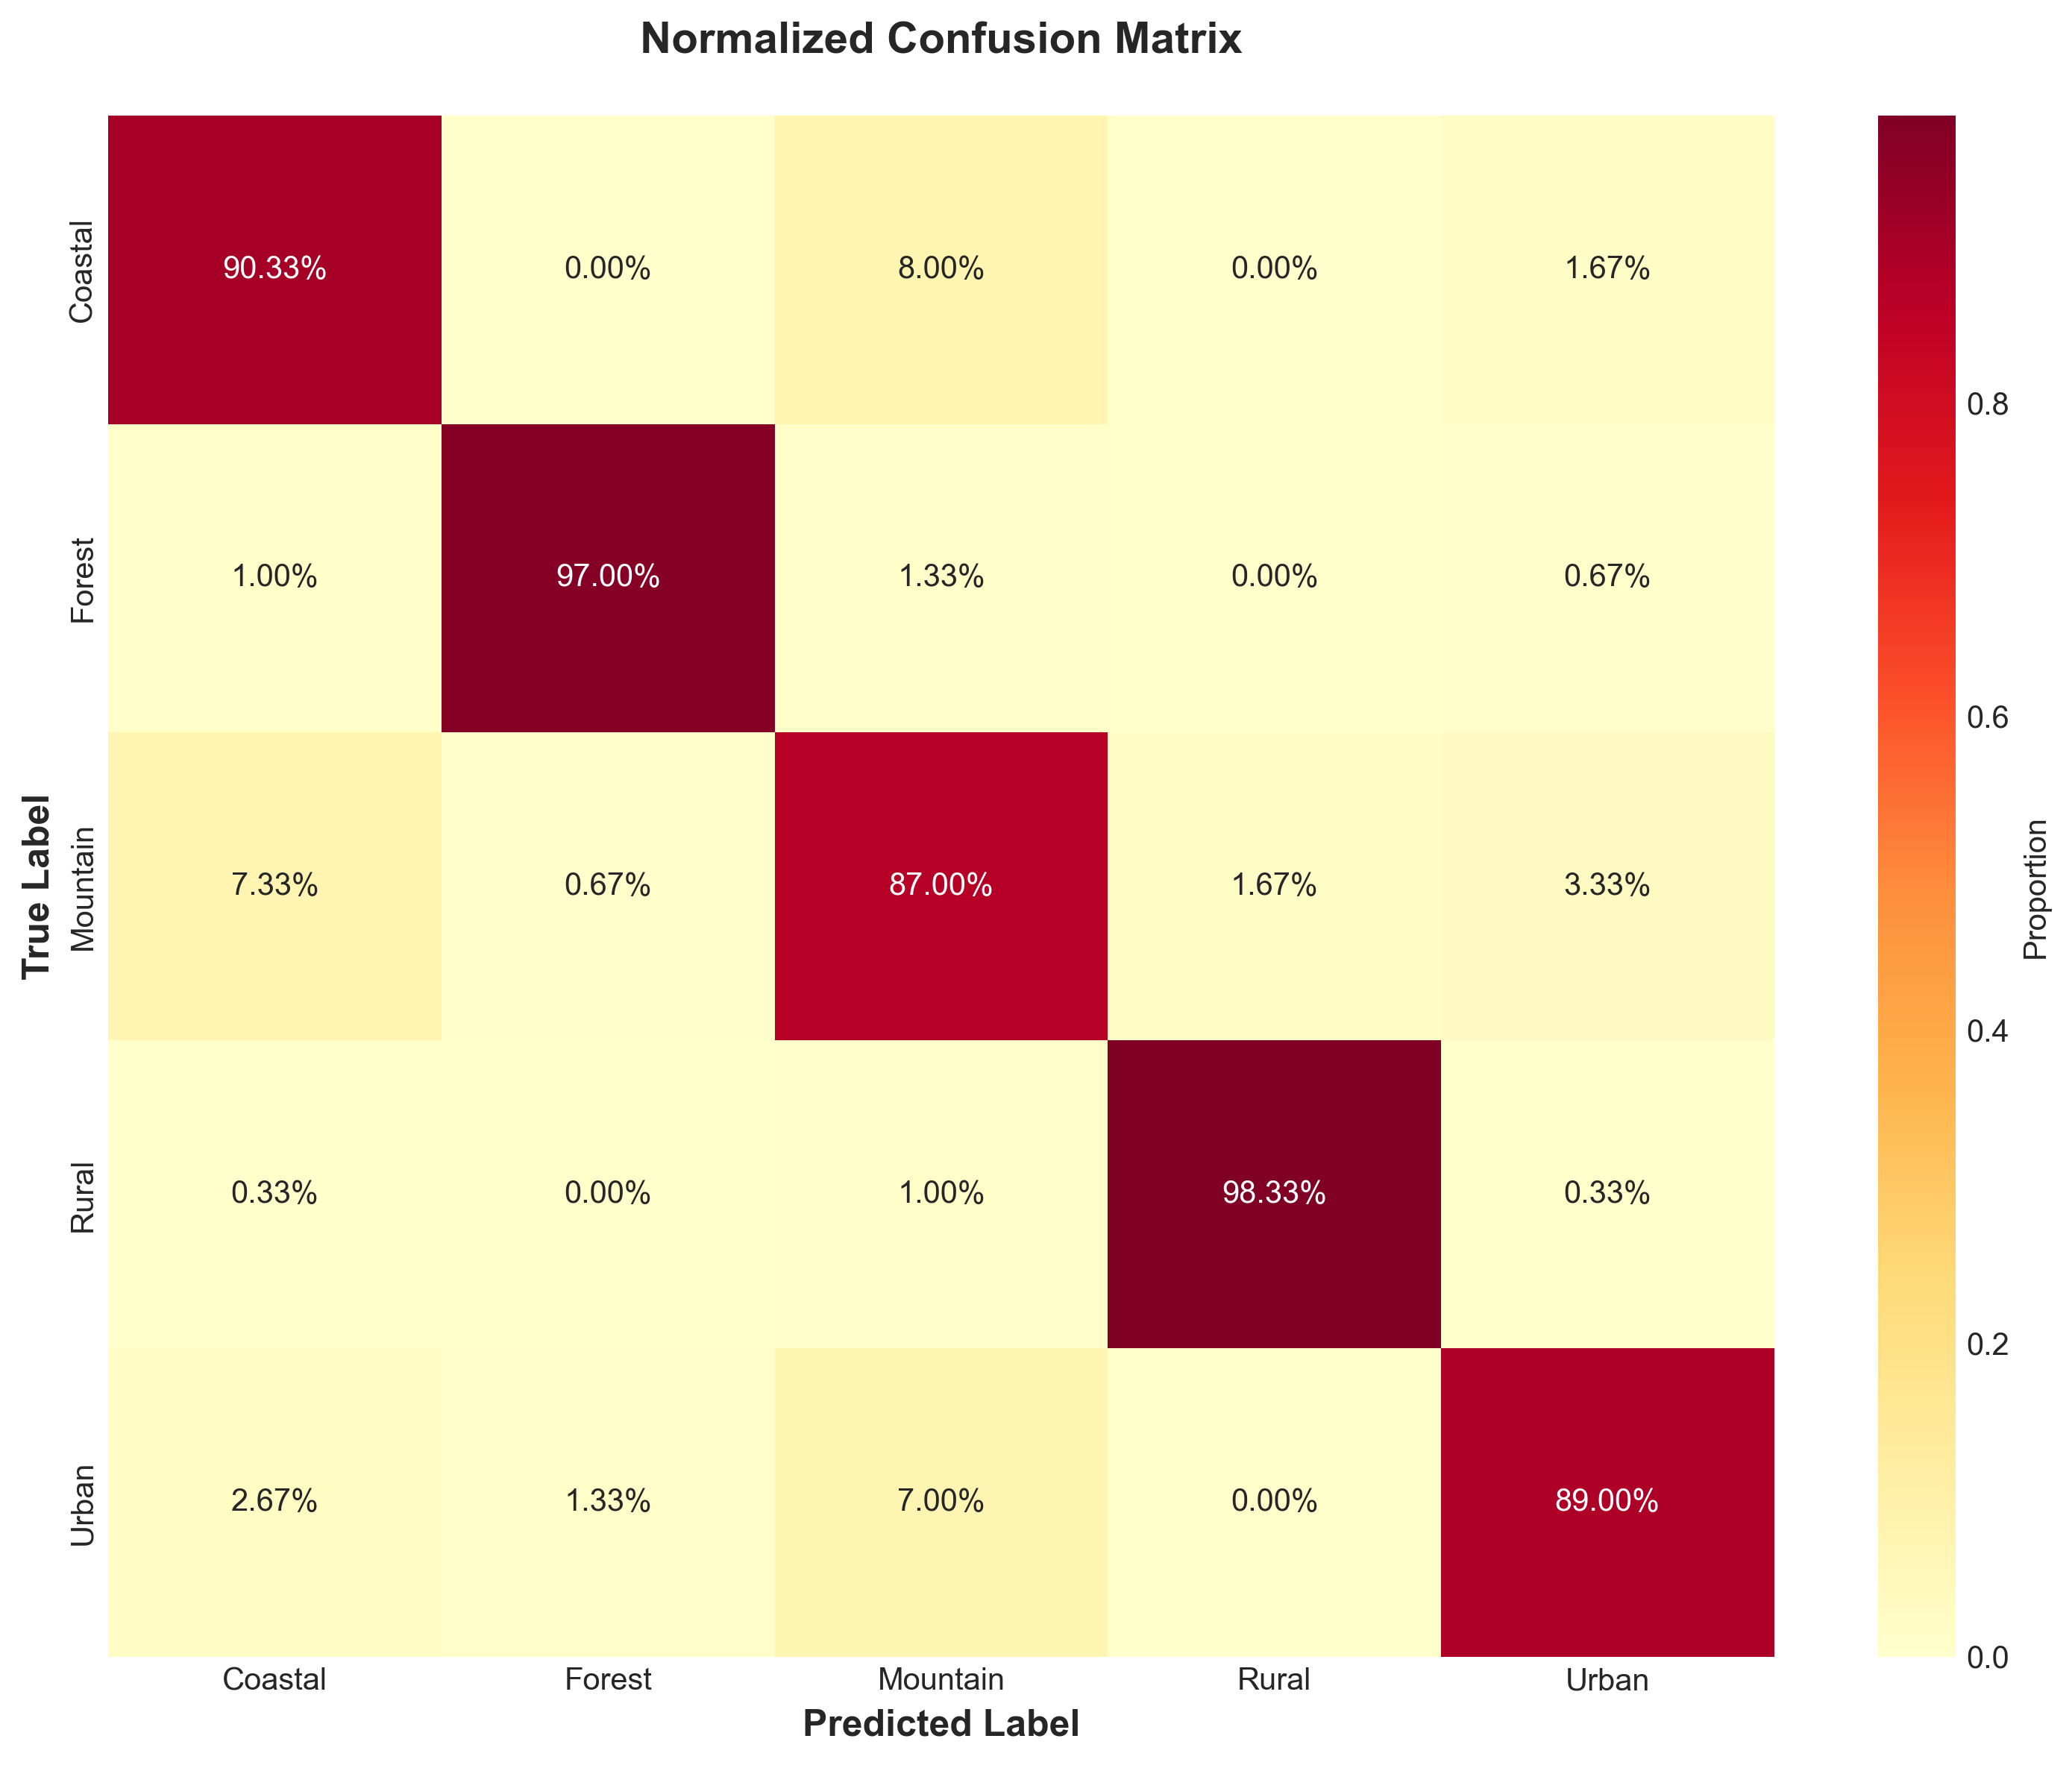
\includegraphics[width=0.78\textwidth]{assets/figures/confusion_matrix_normalized.png}
\caption{Normalized confusion matrix of test predictions}
\label{fig:cm-norm}
\end{figure}
\FloatBarrier

\section{Learning Dynamics}
Training and validation histories show a monotonic decrease in loss and stable improvement in accuracy, with no severe divergence between train and validation trajectories. This suggests controlled optimization and limited overfitting under the selected hyperparameters.

\section{Interpretation of Results}
The achieved macro metrics above 0.92 confirm that broad scene semantics can be learned reliably from visual cues. The current model therefore provides a dependable first-stage signal for location inference pipelines that require robust contextual priors.

From a systems perspective, these results indicate that the baseline has crossed the threshold from experimental prototype to operationally useful semantic module. Strong macro performance combined with interpretable confusion pathways means the model can be trusted as a prior generator for downstream reasoning, provided uncertainty is exposed and handled correctly.

\section{Per-Class Insight Narrative}
\textbf{Coastal:} Performance is strong but affected by overlap with Mountain scenes where shoreline-like rock textures dominate.\newline
\textbf{Forest:} Highest separability suggests consistent feature patterns under current preprocessing policy.\newline
\textbf{Mountain:} Most challenging class, acting as primary boundary stress test for the baseline.\newline
\textbf{Rural:} Highest reliability indicates robust learning of low-density landscape structure.\newline
\textbf{Urban:} High precision shows strong urban feature extraction; recall sensitivity reflects mixed-scene boundaries.

These class wise observations are important because they convert score tables into engineering direction for next-phase improvements.

\section{Limitations}
\begin{itemize}
\item Ambiguity among visually adjacent classes (especially Mountain vs Coastal/Urban).
\item Current output granularity is class-level, not landmark or city-level.
\item Performance may vary under unseen climate/season distributions.
\end{itemize}

Additional limitations include dataset granularity constraints and lack of calibrated uncertainty in current inference output. While softmax confidence is useful, it is not equivalent to calibrated probability under domain shift. This motivates temperature scaling and confidence-reliability analysis in the next phase.

\section{Actionable Lessons Learned}
The project yielded several practical lessons:
\begin{itemize}
\item reproducible split governance is essential for credible comparison,
\item confusion analysis provides more value than aggregate accuracy alone,
\item modular code structure significantly accelerates iteration,
\item stage wise system design lowers risk in ambitious geolocation tasks.
\end{itemize}

\section{Conclusion}
This minor project successfully establishes DeepSceneLoc Stage 1 as a reproducible and high-performing semantic scene classifier for metadata-free location context estimation. With overall accuracy of 92.33\% and balanced macro metrics, the system demonstrates both feasibility and practical readiness for Semester 2 extension toward exact-location prediction.

\section{Report Size Compliance Note}
The report is organized to remain well below the maximum limit of 120 pages while preserving all required chapters, diagrams, tables, and references. Final page count can be verified directly from compiled PDF metadata once the LaTeX engine is available.

